\documentclass[11pt,a4paper]{article}

\usepackage[utf8]{inputenc}
\usepackage[T1]{fontenc}
\usepackage{lmodern}
\usepackage[margin=1in]{geometry}
\usepackage{hyperref}
\usepackage{graphicx}
\usepackage{booktabs}
\usepackage{longtable}
\usepackage{xcolor}
\usepackage{listings}
\usepackage{enumitem}
\usepackage{tikz}
\usetikzlibrary{shapes.geometric, arrows.meta, positioning}

\hypersetup{
  colorlinks=true,
  linkcolor=blue!60!black,
  urlcolor=blue!60!black,
  pdftitle={Codefied Deployment Documentation},
  pdfauthor={Codefied Team}
}

\definecolor{codebg}{RGB}{245,245,245}
\definecolor{codeframe}{RGB}{200,200,200}
\definecolor{commentgreen}{RGB}{0,128,0}

\lstdefinestyle{terminal}{
  backgroundcolor=\color{codebg},
  frame=single,
  rulecolor=\color{codeframe},
  basicstyle=\ttfamily\small,
  breaklines=true,
  columns=fullflexible,
  showstringspaces=false,
  literate={_}{\textunderscore}1
}

\lstdefinestyle{envfile}{
  backgroundcolor=\color{codebg},
  frame=single,
  rulecolor=\color{codeframe},
  basicstyle=\ttfamily\small,
  breaklines=true,
  columns=fullflexible
}

% Redacted deployment identifiers (hashed / masked for documentation)
\newcommand{\maskedectwoip}{\texttt{sha256:54.1\ldots 43.53}}
\newcommand{\maskedvercelurl}{\texttt{https://codefied-****.vercel.app}}
\newcommand{\maskedmongouri}{\texttt{mongodb+srv://[REDACTED\_USER]:[REDACTED\_PASS]@[REDACTED\_CLUSTER].mongodb.net/}}
\newcommand{\maskedgithub}{\texttt{github.com/[REDACTED]/Codefied}}
\newcommand{\maskedpem}{\texttt{[REDACTED]-key.pem}}
\newcommand{\productionip}{\texttt{54.166.43.53}}

\title{\textbf{Codefied --- Production Deployment Documentation}}
\author{Deployment Reference (t3.small PM2 + Nginx Architecture)}
\date{July 2026}

\begin{document}
\maketitle
\tableofcontents
\newpage

\section{Purpose}
This document describes the \textbf{production deployment workflow} for \textbf{Codefied}, an online judge platform, as of \textbf{July 2026}. Production runs on a \textbf{t3.small} EC2 instance with \textbf{PM2} (Node.js backend), \textbf{nginx} (reverse proxy on port~80), and \textbf{Redis in Docker only}---not a full Docker backend stack. It covers infrastructure choices, automation scripts, shell commands, environment configuration, and lessons learned from earlier failed deployments on \texttt{t2.micro}. Sensitive credentials are \textbf{masked or hashed} in summary tables; live examples use the current Elastic IP where helpful.

\section{Architecture Overview}

\subsection{High-Level Topology}
\begin{center}
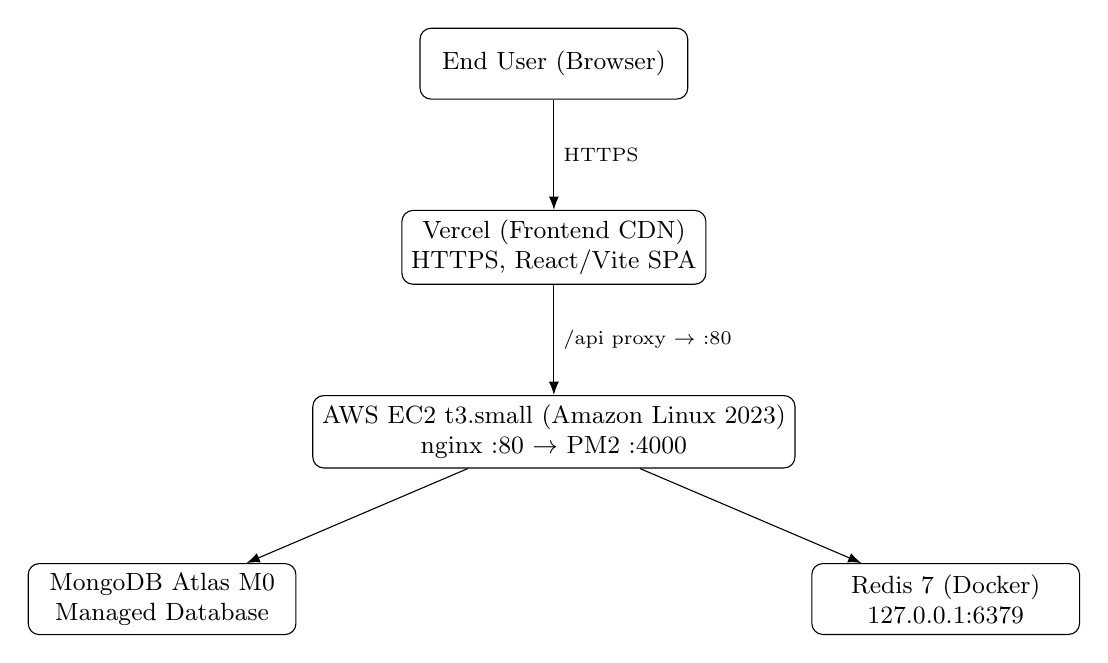
\begin{tikzpicture}[
  node distance=1.4cm,
  box/.style={draw, rounded corners, minimum width=3.4cm, minimum height=0.9cm, align=center, font=\small}
]
  \node[box] (user) {End User (Browser)};
  \node[box, below=of user] (vercel) {Vercel (Frontend CDN)\\HTTPS, React/Vite SPA};
  \node[box, below=of vercel] (ec2) {AWS EC2 t3.small (Amazon Linux 2023)\\nginx :80 $\rightarrow$ PM2 :4000};
  \node[box, below left=1.2cm and 0.2cm of ec2] (atlas) {MongoDB Atlas M0\\Managed Database};
  \node[box, below right=1.2cm and 0.2cm of ec2] (redis) {Redis 7 (Docker)\\127.0.0.1:6379};

  \draw[-{Latex}] (user) -- node[right, font=\scriptsize]{HTTPS} (vercel);
  \draw[-{Latex}] (vercel) -- node[right, font=\scriptsize]{/api proxy $\rightarrow$ :80} (ec2);
  \draw[-{Latex}] (ec2) -- (atlas);
  \draw[-{Latex}] (ec2) -- (redis);
\end{tikzpicture}
\end{center}

\textbf{Key change from earlier docs:} the backend runs as a \textbf{native Node.js process under PM2}, not inside a Docker container. Docker is used \textbf{only for Redis}. nginx listens on port~80 and proxies to \texttt{127.0.0.1:4000}. Port~4000 must \textbf{not} be exposed in the security group.

\subsection{Deployment Targets}
\begin{table}[h]
\centering
\begin{tabular}{@{}lll@{}}
\toprule
\textbf{Component} & \textbf{Platform} & \textbf{Masked Address} \\
\midrule
Frontend (SPA)     & Vercel (Hobby)    & \maskedvercelurl \\
Backend API        & EC2 PM2 + nginx   & \maskedectwoip{} :80 (public) \\
Backend (internal) & PM2 on EC2        & \texttt{127.0.0.1:4000} (localhost only) \\
Redis              & Docker on EC2     & \texttt{127.0.0.1:6379} \\
MongoDB            & Atlas M0 (free)   & \maskedmongouri \\
Source Control     & GitHub            & \maskedgithub \\
\bottomrule
\end{tabular}
\caption{Production service map with redacted identifiers}
\end{table}

\subsection{Why This Split?}
\begin{itemize}[noitemsep]
  \item \textbf{Vercel} hosts the static React build with free HTTPS and global CDN.
  \item \textbf{PM2 on EC2} runs the Express backend natively, saving $\sim$300\,MB RAM versus a Docker backend container.
  \item \textbf{nginx on :80} provides a stable public entry point; Vercel proxies \texttt{/api} to port~80, not :4000.
  \item \textbf{Redis in Docker} powers BullMQ (AI review jobs) and rate limiting, bound to localhost only.
  \item \textbf{MongoDB Atlas M0} provides a free managed database reachable from EC2.
  \item \textbf{1\,GB swap} is mandatory on small instances to prevent OOM freezes under compile/load spikes.
\end{itemize}

\section{Tools and Technologies Used}

\begin{table}[h]
\centering
\begin{tabular}{@{}lp{9.5cm}@{}}
\toprule
\textbf{Tool} & \textbf{Role in Deployment} \\
\midrule
Git / GitHub       & Version control; Vercel auto-deploy on push \\
Vercel             & Frontend hosting, HTTPS, SPA routing, \texttt{/api} reverse proxy \\
AWS EC2            & Backend compute (\texttt{t3.small}, Amazon Linux 2023) \\
AWS Elastic IP     & Static public IPv4 (\productionip) \\
PM2                & Process manager for \texttt{codefied-api} (auto-restart, boot persistence) \\
nginx              & Reverse proxy :80 $\rightarrow$ \texttt{127.0.0.1:4000} \\
Docker Compose     & Runs \texttt{redis} only in production \\
Node.js 20         & Backend runtime (installed via NodeSource RPM) \\
MongoDB Atlas      & Cloud MongoDB (M0 free tier) \\
OpenSSH (\texttt{ssh}) & Remote administration of EC2 \\
\texttt{curl}      & Health checks (\texttt{/api/health}) \\
Vite               & Frontend production build \\
\bottomrule
\end{tabular}
\end{table}

\section{Repository Automation Scripts}

Production setup is automated. Run these from the cloned repo on EC2 (\texttt{/home/ec2-user/codefied}).

\begin{table}[h]
\centering
\begin{tabular}{@{}lp{8.5cm}@{}}
\toprule
\textbf{Script} & \textbf{Purpose} \\
\midrule
\texttt{scripts/setup-t3-small.sh}   & Full first-time setup: swap, packages, Node/PM2, Redis, nginx \\
\texttt{scripts/fix-services.sh}     & Repair Redis, sync \texttt{.env}, restart PM2 and nginx \\
\texttt{scripts/preflight-ec2.sh}    & Pre/post deploy health checks (memory, swap, PM2, nginx, Redis) \\
\texttt{scripts/ec2-optimize.sh}     & Standalone swap tuning (run with \texttt{sudo} if swap missing) \\
\bottomrule
\end{tabular}
\caption{Deployment automation scripts}
\end{table}

\subsection{Key Config Files}
\begin{itemize}[noitemsep]
  \item \texttt{backend/ecosystem.config.cjs} --- PM2 app definition (\texttt{codefied-api}, port~4000, memory limits).
  \item \texttt{deploy/nginx/codefied.conf} --- nginx site config copied to \texttt{/etc/nginx/conf.d/}.
  \item \texttt{frontend/vercel.json} --- SPA rewrites and \texttt{/api} proxy to Elastic IP on port~80.
  \item \texttt{docker-compose.yml} --- \texttt{redis} always; \texttt{backend} under \texttt{profiles: ["docker"]} for local dev only.
\end{itemize}

\section{Pre-Deployment Code Changes}

The following application changes support the current production architecture:

\begin{enumerate}[noitemsep]
  \item Moved secrets from \texttt{docker-compose.yml} into \texttt{.env} files (gitignored).
  \item Added \texttt{FRONTEND\_URL} for dynamic CORS instead of hardcoded \texttt{localhost:5173}.
  \item Centralized refresh-token cookie options; \texttt{COOKIE\_SECURE=true} in production.
  \item Shared Redis configuration via \texttt{backend/utils/redisConfig.js}; production uses \texttt{REDIS\_HOST=127.0.0.1}.
  \item Added \texttt{frontend/vercel.json} proxying \texttt{/api} to \texttt{http://54.166.43.53/api/:path*} (nginx on :80).
  \item Added \texttt{/api/health} endpoint for preflight and external smoke tests.
  \item Backend Docker service moved to \texttt{profiles: ["docker"]} --- not used in production.
  \item Committed \texttt{.env.example} templates (no real secrets).
\end{enumerate}

\section{Environment Variables}

\subsection{Root \texttt{.env} on EC2 (source of truth)}
Create at repo root (\texttt{/home/ec2-user/codefied/.env}). The setup and repair scripts \textbf{copy} this file to \texttt{backend/.env} because PM2's working directory is \texttt{backend/}.

\begin{lstlisting}[style=envfile]
MONGO_URI=<REDACTED_ATLAS_URI>
JWT_ACCESS_SECRET=<REDACTED>
JWT_REFRESH_SECRET=<REDACTED>
GOOGLE_GEMINI_API_KEY=<REDACTED>

# Production (required)
FRONTEND_URL=https://codefied-****.vercel.app
COOKIE_SECURE=true

# PM2 backend talks to Docker Redis on localhost
REDIS_HOST=127.0.0.1
REDIS_PORT=6379
\end{lstlisting}

\textbf{Critical:} After editing \texttt{.env}, run \texttt{cp .env backend/.env} and restart PM2 (\texttt{bash scripts/fix-services.sh} or \texttt{pm2 restart codefied-api}). PM2 does not read the repo-root \texttt{.env} automatically.

\subsection{Vercel Environment Variables}
\begin{lstlisting}[style=envfile]
VITE_API_URL=/api
VITE_APP_URL=https://codefied-****.vercel.app
\end{lstlisting}

\section{Deployment Workflow}

\subsection{Phase 0 --- Prepare Repository}
\begin{lstlisting}[style=terminal]
cd <project-root>
git status
# Ensure .env files are NOT staged
git add .
git commit -m "Prepare Codefied for deployment"
git push origin main
\end{lstlisting}

\subsection{Phase 1 --- MongoDB Atlas}
\begin{enumerate}[noitemsep]
  \item Create or use existing M0 cluster.
  \item Network Access $\rightarrow$ allow \texttt{0.0.0.0/0} (or restrict to Elastic IP \productionip{} only).
  \item Copy connection string into EC2 \texttt{.env} as \texttt{MONGO\_URI}.
\end{enumerate}

\subsection{Phase 2 --- AWS EC2 Backend (t3.small)}

\subsubsection{Launch Instance}
\begin{itemize}[noitemsep]
  \item AMI: \textbf{Amazon Linux 2023} (not Ubuntu)
  \item Instance type: \textbf{\texttt{t3.small}} ($\sim$2\,GB RAM) --- \textbf{not} \texttt{t2.micro}/\texttt{t3.micro}
  \item Elastic IP: allocate and associate \textbf{before} or immediately after launch (\productionip)
  \item Security group inbound:
  \begin{itemize}[noitemsep]
    \item TCP \textbf{22} --- SSH, \textbf{My IP} only (recommended)
    \item TCP \textbf{80} --- \texttt{0.0.0.0/0} (Vercel API proxy + health checks)
    \item \textbf{Do NOT} open TCP \textbf{4000} publicly
  \end{itemize}
  \item Key pair: \maskedpem
\end{itemize}

\subsubsection{SSH into EC2}
\textbf{Important:} Amazon Linux uses \texttt{ec2-user}, not \texttt{ubuntu}.

\begin{lstlisting}[style=terminal]
ssh -i "<path-to-pem>" ec2-user@54.166.43.53
\end{lstlisting}

\subsubsection{Automated Setup (recommended)}
\begin{lstlisting}[style=terminal]
git clone <REDACTED_GITHUB_REPO_URL> ~/codefied
cd ~/codefied
cp .env.example .env
nano .env    # fill secrets; set FRONTEND_URL and COOKIE_SECURE=true

bash scripts/setup-t3-small.sh
\end{lstlisting}

The setup script performs, in order:
\begin{enumerate}[noitemsep]
  \item Preflight RAM check (warns if $<$1.5\,GB --- old micro had 912\,MB)
  \item Creates \textbf{1\,GB swap} with \texttt{vm.swappiness=10}
  \item Installs git, nginx, compilers, Java, Docker, Node.js~20, PM2
  \item Starts Redis: \texttt{docker compose up -d redis}
  \item Copies \texttt{.env} $\rightarrow$ \texttt{backend/.env}; runs \texttt{npm ci}
  \item Starts PM2: \texttt{pm2 start ecosystem.config.cjs}
  \item Deploys nginx: \texttt{deploy/nginx/codefied.conf} $\rightarrow$ \texttt{/etc/nginx/conf.d/}
  \item Runs \texttt{scripts/preflight-ec2.sh}
\end{enumerate}

\subsubsection{Manual Verification}
\begin{lstlisting}[style=terminal]
# PM2 backend (localhost only)
curl http://127.0.0.1:4000/api/health

# nginx proxy (public path)
curl http://127.0.0.1/api/health
curl http://54.166.43.53/api/health

pm2 status
pm2 logs codefied-api --lines 30 --nostream
docker ps --filter name=codefied-redis
\end{lstlisting}

Expected health response: JSON with status OK from \texttt{/api/health}.

\subsection{Phase 3 --- Vercel Frontend}

\subsubsection{\texttt{frontend/vercel.json}}
Traffic goes to nginx on \textbf{port~80}, not :4000:

\begin{lstlisting}[style=envfile]
{
  "rewrites": [
    {
      "source": "/api/:path*",
      "destination": "http://54.166.43.53/api/:path*"
    },
    {
      "source": "/(.*)",
      "destination": "/index.html"
    }
  ]
}
\end{lstlisting}

\subsubsection{Vercel Project Settings}
\begin{itemize}[noitemsep]
  \item Root Directory: \texttt{frontend}
  \item Build Command: \texttt{npm run build}
  \item Output Directory: \texttt{dist}
  \item Env: \texttt{VITE\_API\_URL=/api}, \texttt{VITE\_APP\_URL=<vercel-url>}
\end{itemize}

\subsection{Phase 4 --- Connect Frontend and Backend}
After Vercel deploy, ensure EC2 \texttt{.env} matches the live frontend URL:
\begin{lstlisting}[style=envfile]
FRONTEND_URL=https://codefied-****.vercel.app
COOKIE_SECURE=true
\end{lstlisting}

Sync into backend and restart:
\begin{lstlisting}[style=terminal]
cd ~/codefied
cp .env backend/.env
bash scripts/fix-services.sh
# or: pm2 restart codefied-api && sudo systemctl restart nginx
\end{lstlisting}

\subsection{Phase 5 --- Elastic IP}
See Section~\ref{sec:elastic-ip}. The current production Elastic IP is \productionip. Vercel \texttt{vercel.json} must match this address. If the EIP changes, update \texttt{vercel.json}, commit, push, and wait for Vercel redeploy.

\section{AWS Elastic IP --- Detailed Guide}
\label{sec:elastic-ip}

\subsection{What Is an Elastic IP?}
An \textbf{Elastic IP (EIP)} is a static, public IPv4 address allocated to your AWS account. When associated with an EC2 instance, the address persists across \textbf{stop/start} and \textbf{reboot} cycles.

\subsection{Why Codefied Needs It}
The Vercel frontend proxies API traffic to the backend using the Elastic IP in \texttt{frontend/vercel.json}:
\begin{lstlisting}[style=envfile]
"destination": "http://54.166.43.53/api/:path*"
\end{lstlisting}
nginx on the instance listens on port~80 and forwards to PM2 on :4000. If the EC2 public IP changes without updating \texttt{vercel.json}, the proxy breaks.

\subsection{Prerequisites}
\begin{itemize}[noitemsep]
  \item EC2 \texttt{t3.small} instance running in the target region (e.g.\ \texttt{us-east-1}).
  \item Backend verified: \texttt{curl http://127.0.0.1:4000/api/health} and \texttt{curl http://54.166.43.53/api/health} succeed.
  \item Security group allows TCP \textbf{80} inbound (not 4000).
\end{itemize}

\subsection{Step-by-Step: AWS Console}
\begin{enumerate}
  \item Open \textbf{EC2 Dashboard} in the \textbf{same region} as your instance.
  \item Navigate to \textbf{Network \& Security} $\rightarrow$ \textbf{Elastic IPs}.
  \item Click \textbf{Allocate Elastic IP address} $\rightarrow$ \textbf{Allocate}.
  \item Select the EIP $\rightarrow$ \textbf{Actions} $\rightarrow$ \textbf{Associate Elastic IP address}.
  \begin{itemize}[noitemsep]
    \item Resource type: \textbf{Instance}.
    \item Instance: select the Codefied EC2 instance.
  \end{itemize}
  \item Click \textbf{Associate}. Production EIP (masked in tables): \maskedectwoip.
\end{enumerate}

\subsection{Post-Association: Update Vercel Proxy}
If the Elastic IP differs from \texttt{vercel.json}:
\begin{enumerate}[noitemsep]
  \item Edit \texttt{frontend/vercel.json} $\rightarrow$ update the \texttt{/api} \texttt{destination} host.
  \item Commit and push to GitHub.
  \item Wait for Vercel auto-redeploy.
  \item Test: \texttt{curl http://<ELASTIC\_IP>/api/health}
\end{enumerate}

\subsection{Elastic IP Billing Rules}
\begin{table}[h]
\centering
\begin{tabular}{@{}ll@{}}
\toprule
\textbf{Scenario} & \textbf{Charge} \\
\midrule
EIP attached to a \textbf{running} instance & Free \\
EIP attached to a \textbf{stopped} instance & Hourly charge applies \\
EIP allocated but \textbf{not associated} & Hourly charge applies \\
\bottomrule
\end{tabular}
\caption{AWS Elastic IP cost behaviour (verify current AWS pricing)}
\end{table}

\section{Useful Operational Commands}

\subsection{Local Development (Windows) --- Optional Docker Backend}
For local dev, use the Docker backend profile instead of PM2:
\begin{lstlisting}[style=terminal]
docker compose --profile docker up -d redis backend
cd frontend
npm run dev
\end{lstlisting}

Production EC2 uses PM2 only; the \texttt{docker} profile is \textbf{not} started on the server.

\subsection{EC2 Backend Updates (git pull workflow)}
\begin{lstlisting}[style=terminal]
cd ~/codefied
git pull

# Sync env if changed
cp .env backend/.env

cd backend
npm ci --omit=dev    # if package-lock.json changed

pm2 restart codefied-api
pm2 logs codefied-api --lines 50 --nostream

# If nginx config changed
sudo cp deploy/nginx/codefied.conf /etc/nginx/conf.d/codefied.conf
sudo nginx -t && sudo systemctl restart nginx

# Full repair if something is broken
cd ~/codefied && bash scripts/fix-services.sh
\end{lstlisting}

\subsection{PM2 Day-to-Day}
\begin{lstlisting}[style=terminal]
pm2 status
pm2 logs codefied-api              # live tail
pm2 logs codefied-api --lines 100 --nostream
pm2 restart codefied-api
pm2 stop codefied-api
pm2 save                           # persist process list across reboot
\end{lstlisting}

\subsection{Redis (Docker)}
\begin{lstlisting}[style=terminal]
cd ~/codefied
docker compose up -d redis
docker compose ps
docker logs codefied-redis --tail 30
\end{lstlisting}

\subsection{Preflight and Health Checks}
\begin{lstlisting}[style=terminal]
bash scripts/preflight-ec2.sh

# Internal
curl http://127.0.0.1:4000/api/health
curl http://127.0.0.1/api/health

# External (requires SG port 80)
curl http://54.166.43.53/api/health

# Login smoke test (expect 401 for bad credentials, NOT 500)
curl -X POST http://54.166.43.53/api/auth/login \
  -H "Content-Type: application/json" \
  -H "Origin: https://codefied-****.vercel.app" \
  -d '{"identifier":"test","password":"test"}'

# Verify env loaded by PM2 process
grep FRONTEND_URL backend/.env
\end{lstlisting}

\section{Issues and Challenges Encountered}

\subsection{Lessons from the Old \texttt{t2.micro} Deployment}
The first production attempt on a \textbf{912\,MB \texttt{t2.micro}} with \textbf{zero swap} and a \textbf{full Docker backend} failed repeatedly. The current architecture exists specifically to avoid these mistakes.

\begin{longtable}{@{}p{3.2cm}p{4.2cm}p{6.8cm}@{}}
\toprule
\textbf{Issue} & \textbf{Symptom} & \textbf{Resolution} \\
\midrule
\endhead
\texttt{t2.micro} OOM &
SSH hangs; instance unresponsive; compile jobs kill Node &
Upgrade to \texttt{t3.small}; add \textbf{1\,GB swap}; use PM2 not Docker backend \\
\addlinespace
Docker backend RAM overhead &
$\sim$300\,MB extra for container; builds OOM on micro &
Run backend via PM2; Docker for Redis only \\
\addlinespace
No swap configured &
Sudden freeze under memory spike; no recovery without reboot &
\texttt{setup-t3-small.sh} creates 1\,GB swap; \texttt{ec2-optimize.sh} as fallback \\
\addlinespace
\texttt{.env} not loaded by PM2 &
Login 500; CORS errors; \texttt{FRONTEND\_URL} still localhost &
\texttt{cp .env backend/.env}; \texttt{pm2 restart codefied-api} or \texttt{fix-services.sh} \\
\addlinespace
nginx not started &
External \texttt{curl} to :80 fails; Vercel API proxy 502/timeout &
\texttt{sudo systemctl enable nginx}; \texttt{sudo systemctl restart nginx}; verify \texttt{codefied.conf} \\
\addlinespace
Port 4000 exposed publicly &
Unnecessary attack surface; bypasses nginx &
Remove SG rule for :4000; only open :22 (My IP) and :80 (0.0.0.0/0) \\
\addlinespace
Wrong SSH user &
\texttt{Permission denied (publickey)} with \texttt{ubuntu@} &
Use \texttt{ec2-user@} for Amazon Linux 2023 \\
\addlinespace
Vercel build failure &
\texttt{Cannot find package '@tailwindcss/vite'} &
Move Tailwind deps into \texttt{frontend/package.json}; add \texttt{esbuild} \\
\addlinespace
Commented env lines &
Production vars inactive on EC2 &
Uncomment \texttt{FRONTEND\_URL}; set \texttt{COOKIE\_SECURE=true} \\
\addlinespace
Mixed content (avoided) &
HTTPS site cannot call HTTP API directly &
Proxy \texttt{/api} through Vercel to EC2 :80 via nginx \\
\bottomrule
\caption{Deployment troubleshooting log (July 2026)}
\end{longtable}

\section{Security Checklist}
\begin{itemize}[noitemsep]
  \item Never commit \texttt{.env} files.
  \item Rotate MongoDB password and Gemini API key if previously exposed.
  \item Use strong random \texttt{JWT\_ACCESS\_SECRET} and \texttt{JWT\_REFRESH\_SECRET}.
  \item Restrict EC2 SSH (port 22) to your IP.
  \item \textbf{Do not} expose port 4000 in the security group.
  \item Redis bound to \texttt{127.0.0.1:6379} only (see \texttt{docker-compose.yml}).
  \item Set \texttt{COOKIE\_SECURE=true} in production.
  \item Document masked addresses only in internal docs.
\end{itemize}

\section{Cost Summary (July 2026)}
\begin{table}[h]
\centering
\begin{tabular}{@{}ll@{}}
\toprule
\textbf{Service} & \textbf{Typical Cost} \\
\midrule
Vercel Hobby           & Free \\
AWS EC2 \texttt{t3.small} & $\sim$\$15--17/month (not free tier) \\
MongoDB Atlas M0       & Free \\
Redis (Docker on EC2)  & Included in EC2 \\
Elastic IP (attached, running) & Free \\
nginx + PM2            & Included in EC2 \\
\bottomrule
\end{tabular}
\end{table}

\section{Quick Deployment Checklist}
\begin{enumerate}
  \item Rotate secrets; push code to GitHub (no \texttt{.env}).
  \item Configure MongoDB Atlas network access.
  \item Launch \textbf{\texttt{t3.small}} EC2; allocate Elastic IP (\productionip).
  \item Security group: port \textbf{22} (My IP), port \textbf{80} (0.0.0.0/0); \textbf{no} port 4000.
  \item SSH as \texttt{ec2-user}; clone repo; create root \texttt{.env}.
  \item Run \texttt{bash scripts/setup-t3-small.sh} (swap + PM2 + nginx + Redis).
  \item Verify \texttt{bash scripts/preflight-ec2.sh} passes.
  \item Confirm \texttt{frontend/vercel.json} points to \texttt{http://54.166.43.53/api/:path*}.
  \item Deploy frontend on Vercel; set \texttt{VITE\_*} env vars.
  \item Set \texttt{FRONTEND\_URL} and \texttt{COOKIE\_SECURE=true}; run \texttt{fix-services.sh}.
  \item End-to-end test: register, login, code run, AI review.
\end{enumerate}

\appendix
\section{Deployment Cheat Sheet}
\label{appendix:cheatsheet}

\subsection{Masked Production Map}
\begin{table}[h]
\centering
\small
\begin{tabular}{@{}ll@{}}
\toprule
\textbf{What} & \textbf{Masked Value} \\
\midrule
Frontend URL       & \maskedvercelurl \\
Backend (public)   & \maskedectwoip{} :80 \\
Backend (internal) & \texttt{127.0.0.1:4000} \\
Elastic IP (live)  & \productionip \\
SSH user           & \texttt{ec2-user} \\
SSH key            & \maskedpem \\
GitHub repo        & \maskedgithub \\
MongoDB            & \maskedmongouri \\
PM2 app name       & \texttt{codefied-api} \\
\bottomrule
\end{tabular}
\end{table}

\subsection{One-Page Command Reference}

\subsubsection{SSH (from Windows PowerShell)}
\begin{lstlisting}[style=terminal]
ssh -i "<path-to-pem>" ec2-user@54.166.43.53
\end{lstlisting}

\subsubsection{First-Time Setup (EC2)}
\begin{lstlisting}[style=terminal]
cd ~/codefied
cp .env.example .env && nano .env
bash scripts/setup-t3-small.sh
\end{lstlisting}

\subsubsection{Start / Restart Backend (EC2)}
\begin{lstlisting}[style=terminal]
cd ~/codefied
docker compose up -d redis                    # Redis only
cp .env backend/.env                          # sync env before PM2 restart
pm2 restart codefied-api
pm2 logs codefied-api --lines 30 --nostream

# Full repair (Redis + env + PM2 + nginx)
bash scripts/fix-services.sh
\end{lstlisting}

\subsubsection{Health Checks}
\begin{lstlisting}[style=terminal]
bash scripts/preflight-ec2.sh
curl http://127.0.0.1:4000/api/health
curl http://54.166.43.53/api/health
pm2 status
sudo systemctl status nginx
\end{lstlisting}

\subsubsection{Git + Vercel (local machine)}
\begin{lstlisting}[style=terminal]
git add .
git status                    # confirm no .env staged
git commit -m "message"
git push origin main          # triggers Vercel redeploy
\end{lstlisting}

\subsubsection{Frontend Local Dev (Windows)}
\begin{lstlisting}[style=terminal]
docker compose --profile docker up -d redis backend
cd frontend
npm run dev
\end{lstlisting}

\subsection{Environment Variables at a Glance}

\subsubsection{EC2 root \texttt{.env} (production)}
\begin{table}[h]
\centering
\small
\begin{tabular}{@{}ll@{}}
\toprule
\textbf{Variable} & \textbf{Production Value} \\
\midrule
\texttt{MONGO\_URI}           & Atlas connection string (secret) \\
\texttt{JWT\_ACCESS\_SECRET}  & Long random string (secret) \\
\texttt{JWT\_REFRESH\_SECRET}  & Long random string (secret) \\
\texttt{GOOGLE\_GEMINI\_API\_KEY} & Gemini key (secret) \\
\texttt{FRONTEND\_URL}        & \maskedvercelurl \\
\texttt{COOKIE\_SECURE}       & \texttt{true} \\
\texttt{REDIS\_HOST}          & \texttt{127.0.0.1} \\
\texttt{REDIS\_PORT}          & \texttt{6379} \\
\bottomrule
\end{tabular}
\end{table}

\textbf{Remember:} copy to \texttt{backend/.env} before restarting PM2.

\subsubsection{Vercel dashboard}
\begin{table}[h]
\centering
\small
\begin{tabular}{@{}ll@{}}
\toprule
\textbf{Variable} & \textbf{Value} \\
\midrule
\texttt{VITE\_API\_URL} & \texttt{/api} \\
\texttt{VITE\_APP\_URL} & \maskedvercelurl \\
\bottomrule
\end{tabular}
\end{table}

\subsection{Security Group Ports}
\begin{table}[h]
\centering
\small
\begin{tabular}{@{}llll@{}}
\toprule
\textbf{Port} & \textbf{Protocol} & \textbf{Source} & \textbf{Purpose} \\
\midrule
22   & TCP & My IP (recommended) & SSH \\
80   & TCP & 0.0.0.0/0           & nginx $\rightarrow$ PM2 (Vercel proxy) \\
4000 & --- & \textbf{Do not open} & PM2 localhost only \\
\bottomrule
\end{tabular}
\end{table}

\subsection{PM2 Configuration (\texttt{ecosystem.config.cjs})}
\begin{lstlisting}[style=envfile]
apps: [{
  name: "codefied-api",
  script: "server.js",
  cwd: backend/,
  PORT: 4000,
  max_memory_restart: "450M",
  NODE_OPTIONS: "--max-old-space-size=384"
}]
\end{lstlisting}

\subsection{Nginx Configuration (\texttt{deploy/nginx/codefied.conf})}
nginx listens on port~80 and proxies all traffic (including \texttt{/api/health}) to \texttt{127.0.0.1:4000}. Installed to \texttt{/etc/nginx/conf.d/codefied.conf}; default site removed.

\subsection{Deploy / Fix Decision Tree}
\begin{center}
\small
\begin{tabular}{@{}p{4.5cm}p{7.8cm}@{}}
\toprule
\textbf{Symptom} & \textbf{First Action} \\
\midrule
Cannot SSH &
Try \texttt{ec2-user@} not \texttt{ubuntu@}; check key path and SG port 22 \\
\addlinespace
Instance frozen / OOM &
Check swap (\texttt{free -m}); upgrade to \texttt{t3.small}; \texttt{sudo bash scripts/ec2-optimize.sh} \\
\addlinespace
Backend down on :4000 &
\texttt{pm2 logs codefied-api}; verify \texttt{backend/.env}; \texttt{bash scripts/fix-services.sh} \\
\addlinespace
:4000 OK but :80 fails &
\texttt{sudo systemctl status nginx}; \texttt{sudo nginx -t}; redeploy \texttt{codefied.conf} \\
\addlinespace
Vercel API 502/timeout &
Check SG port 80; \texttt{curl http://54.166.43.53/api/health}; verify EIP in \texttt{vercel.json} \\
\addlinespace
Login returns 500 &
Set \texttt{FRONTEND\_URL}; \texttt{cp .env backend/.env}; \texttt{pm2 restart codefied-api} \\
\addlinespace
Redis connection errors &
\texttt{docker compose up -d redis}; confirm \texttt{REDIS\_HOST=127.0.0.1} \\
\addlinespace
IP changed after stop/start &
Allocate Elastic IP; update \texttt{vercel.json}; redeploy Vercel \\
\bottomrule
\end{tabular}
\end{center}

\subsection{End-to-End Smoke Test (Production)}
\begin{enumerate}[noitemsep]
  \item \texttt{bash scripts/preflight-ec2.sh} $\rightarrow$ \textbf{PASSED}
  \item \texttt{curl http://54.166.43.53/api/health} $\rightarrow$ 200 OK
  \item Open \maskedvercelurl
  \item Register new account
  \item Login
  \item Run code in Code Runner (Python: \texttt{print("hello")})
  \item Open Problems page
  \item Submit a solution or trigger AI review
\end{enumerate}

\vfill
\begin{center}
\small\textit{Document generated for Codefied deployment (July 2026). Production: t3.small, PM2 + nginx, Redis-in-Docker. Live credentials are intentionally redacted in summary tables.}
\end{center}

\end{document}